%======================================================================
% Poznamky_7_identicke_castice.pdf
%======================================================================
\section{Systémy několika identických částic -- fyzika}
\strana{I1}

\kw{identické částice} $\to$ všechny vlastnosti stejné
\begin{itemize}[nosep]
  \item[--] Hamiltonián symetrický vůči záměně $i\leftrightarrow j$
\end{itemize}
např.:
\[
  H = \frac{p_1^2}{2m} + \frac{p_2^2}{2m} + V_{\text{int}}\big(|\vec r_1 - \vec r_2|\big) + V_{\text{ext}}(\vec r_1) + V_{\text{ext}}(\vec r_2)
\]
v QM hlubší důsledky než v klas. Např.\ částice nelze identifikovat podle trajektorie.

\kw{nerozlišitelnost}: žádným měřením nelze rozhodnout, o kterou částici jde

\subsection*{Výměnná (permutační) symetrie}
operace symetrie -- záměna $i\leftrightarrow j$ $\to$ unitární operátor \\
\kw{permutační operátor} $P_{ij}$

\begin{priklad}[Př: dvě částice]
$\mathcal{H} = \mathcal{H}_1\otimes\mathcal{H}_2$ \\
nerozlišitelnost \dots\ izomorfie $\mathcal{H}_1\equiv\mathcal{H}_2\equiv\mathcal{H}$ \\
nechť: částice 1 je ve stavu $\ket{\alpha}\in\mathcal{H}$ \\
\phantom{nechť:} částice 2 \phantom{je} ve stavu $\ket{\beta}\in\mathcal{H}$ \quad \dots\ $\ket{\psi} = \ket{\alpha}\ket{\beta}$

def: \quad $P_{12}\ket{\alpha}\ket{\beta} = \ket{\beta}\ket{\alpha}$ \\
podob.\ na složené stavy \quad
$P_{12}\sum_{\alpha\beta}c_{\alpha\beta}\ket{\alpha}\ket{\beta} = \sum_{\alpha\beta}c_{\alpha\beta}\ket{\beta}\ket{\alpha} = \sum_{\alpha\beta}c_{\beta\alpha}\ket{\alpha}\ket{\beta}$

$x$-reprezentace:
\begin{align*}
  P_{12}\int\psi(x_1,x_2)\ket{x_1}\ket{x_2}\,\dd x_1\dd x_2 &= \int\psi(x_1,x_2)\ket{x_2}\ket{x_1}\,\dd x_1\dd x_2 \\
  \dots\ \text{přeznačení integ.\ prom.\ } x_1\leftrightarrow x_2 &= \int\psi(x_2,x_1)\ket{x_1}\ket{x_2}\,\dd x_1\dd x_2
\end{align*}
tj.\ \quad $P_{12}\psi(x_1,x_2) = \psi(x_2,x_1)$
\end{priklad}

\underline{vl.\ vektory $P_{12}$:} \quad $P_{12}^2 = I$ \quad $\Rightarrow$ \quad $\lambda = \pm1$ \dots\ vl.\ č.
\begin{align*}
  \lambda = 1 &\quad\dots\quad \psi(x_1,x_2) = \psi(x_2,x_1) \quad\dots\ \text{symetrie } c_{\alpha\beta} = c_{\beta\alpha} \\
  \lambda = -1 &\quad\dots\quad \psi(x_1,x_2) = -\psi(x_2,x_1) \quad\dots\ \text{antisymetrie } c_{\alpha\beta} = -c_{\beta\alpha}
\end{align*}

\underline{symetrie $H$:} \quad $P_{12}HP_{12} = H$ \quad tj.\ $[P_{12},H] = 0$ \dots\ společné vl.\ v. \\
\quad tj.\ $\forall$ vl.\ stav $H$ lze volit buď sym.\ nebo antisym. \\
\quad (nemusí být degenerace)

\underline{více částic:} \quad problém \quad $[P_{12},P_{23}]\neq 0$ \quad atd.
\quad \pozn{$P_{12}P_{23}\ket{123} = \ket{312}$, \ $P_{23}P_{12}\ket{123} = \ket{231}$} \\
\dots\ nelze volit společnou úplnou množinu \sout{vektorů} vl.\ vektorů, \\
ale invariantní podprostory:

%----------------------------------------------------------------------
\strana{I2}
\begin{priklad}[Př: invariantní podprostory pro 3 částice]
\begin{itemize}
  \item totál.\ symetrický (1D) / antisymetrický
  \[
    \tfrac{1}{\sqrt6}\big\{\ket{\alpha\beta\gamma} + \ket{\beta\gamma\alpha} + \ket{\gamma\alpha\beta} \pm \ket{\gamma\beta\alpha} \pm \ket{\beta\alpha\gamma} \pm \ket{\alpha\gamma\beta}\big\}
    \qquad \pozn{$P_\forall\ (\pm)$}
  \]
  \item 2D:
  \[
  \begin{array}{r@{\,}c@{\ }c@{\ }c@{\ }c@{\ }c@{\ }c@{\ }l}
    \frac{1}{\sqrt{12}}\big\{ & 2\ket{\alpha\beta\gamma} & +2\ket{\beta\alpha\gamma} & -\ket{\alpha\gamma\beta} & -\ket{\gamma\alpha\beta} & -\ket{\beta\gamma\alpha} & -\ket{\gamma\beta\alpha} & \big\}\quad P_{12}\,(+) \\[3pt]
    \frac12\big\{ & 0 & 0 & +\ket{\alpha\gamma\beta} & -\ket{\gamma\alpha\beta} & +\ket{\beta\gamma\alpha} & -\ket{\gamma\beta\alpha} & \big\}\quad P_{12}\,(-)
  \end{array}
  \]
  \item 2D:
  \[
  \begin{array}{r@{\,}c@{\ }c@{\ }c@{\ }c@{\ }c@{\ }c@{\ }l}
    \frac{1}{\sqrt{12}}\big\{ & 2\ket{\alpha\beta\gamma} & -2\ket{\beta\alpha\gamma} & +\ket{\alpha\gamma\beta} & -\ket{\gamma\alpha\beta} & +\ket{\gamma\beta\alpha} & -\ket{\beta\gamma\alpha} & \big\}\quad P_{12}\,(-) \\[3pt]
    \frac12\big\{ & 0 & 0 & + & + & - & - & \big\}\quad P_{12}\,(+)
  \end{array}
  \]
\end{itemize}
\end{priklad}

Permutační operátory míchají vektory z invar.\ prostoru jen mezi sebou, \\
navíc $\forall$ komutují s $H$ \quad $\to$ vl.\ v.\ $H$ lze konstr.\ z vl.\ podprostorů, \\
\hspace*{5.5cm} navíc čas.\ vývoj ponechává vl.\ podprostory

\underline{naštěstí:} uvidíme, že jen tot.\ sym.\ / tot.\ antisym.\ jsou povoleny

\sout{Nerozlišitelnost}: \underline{Ostatní pozorovatelné}: \quad
(příklad: pozitronium $e^-e^+$, $H$ invar.\ $e^+\leftrightarrow e^-$, ale rozliš.) \\
nerozlišitelnost $\to$ žádné měření nerozliší $\ket{\psi}$ a $P_{ij}\ket{\psi}$ \\
\quad tj.\ \quad $\mel{\psi}{P_{ij}AP_{ij}}{\psi} = \mel{\psi}{A}{\psi}\ \ \forall\ket{\psi}$ \quad $\Rightarrow$ \quad $[A,P_{ij}] = 0$ \\
$\to$ $\forall$ pozorovatelné jsou invar.\ vůči permutacím

\pozor{vlastní podprostory se nemíchají!} \\
např.: \quad $P_{ij}\ket{s} = \ket{s}$, \quad $P_{ij}\ket{a} = -\ket{a}$ \quad $\Rightarrow$ \quad $\mel{s}{A}{a} = -\mel{s}{A}{a} = 0$ \\
\quad tj.\ pro $\ket{\psi} = \alpha\ket{s} + \beta\ket{a}$ je $\mel{\psi}{A}{\psi} = |\alpha|^2\mel{s}{A}{s} + |\beta|^2\mel{a}{A}{a}$ \\
$\to$ interference není pozorovatelná \quad \dots\ \kw{superselekční pravidlo} \\
\hspace*{6cm} (výběrová prav.\ je pro $H$; proto super)

\begin{veta}[Symetrizační postulát]
V přírodě nastává jen jeden z těchto případů:
\begin{enumerate}[label=(\alph*)]
  \item částice má celočíselný spin a její mnohočásticové stavy jsou totálně symetrické \dots\ \kw{BOSON} \dots\ Bose--Einstein statistika
  \item částice má poločíselný spin a její mnohočásticové stavy jsou totálně antisymetrické \dots\ \kw{FERMION} \dots\ Fermi--Dirac st.
\end{enumerate}
\end{veta}

\begin{veta}[Důsledek: Pauliho vylučovací princip]
dva nerozlišitelné fermiony nemohou být ve stejném stavu.
\end{veta}

%----------------------------------------------------------------------
\strana{I3}
\subsection*{Příklad: dvouelektronové systémy}
Předp., že $[H,S] = 0$, kde $S = S_1 + S_2$ je celkový spin

Potom vl.\ stavy $H$ separované: \quad
$\ket{\psi} = \underbrace{\ket{\phi}}_{\text{prostor.\ část}}\underbrace{\ket{\chi}}_{\text{spin.\ část}}$

kde $\ket{\chi}$ lze volit jako vl.\ stav $S^2, S_z$, tj.\ (viz skládání m.\ hybn.)
\[
  \ket{\chi} = \begin{cases}
    S = 1: & \left.\begin{array}{l}
               \ket{++} \\
               \frac{1}{\sqrt2}\big(\ket{+-} + \ket{-+}\big) \\
               \ket{--}
             \end{array}\right\}
             \ \text{\uv{triplet}}\dots\text{symetrický}\quad P_{12}\underbrace{\ket{\chi}}_{\ket{1m}} = \ket{\chi} \\[18pt]
    S = 0: & \ \frac{1}{\sqrt2}\big(\ket{+-} - \ket{-+}\big)
             \quad\dots\ \text{\uv{singlet}}\dots\text{antisym.}\quad P_{12}\ket{\chi} = -\ket{\chi}
  \end{cases}
\]

\begin{itemize}
  \item triplet je symetrický, neboť $S_\pm = S_{1\pm} + S_{2\pm}$ komutují s $P_{12}$ a stav $\ket{++}$ je symetrický.
  \item permutační operátor lze faktorizovat \quad $P_{12} = P_{12}^{(x)}P_{12}^{(s)}$, kde \\
        spinová část \quad $P_{12}^{(s)} = \frac12\Big(I + \frac{4}{\hbar^2}\vec S_1\cdot\vec S_2\Big)$, \quad
        neboť vl.\ č.\ $S_1\cdot S_2 = \begin{cases} \frac{\hbar^2}{4} & \text{triplet} \\ -\frac34\hbar^2 & \text{singlet}\end{cases}$
\end{itemize}
\[
  P_{12}\ket{\phi}\ket{\chi} = P_{12}^{(x)}\ket{\phi}\,P_{12}^{(s)}\ket{\chi}
\]
$\ket{\psi}$ musí být totálně antisym. \quad $\Rightarrow$ \quad
$\begin{cases} \ket{\phi}\ \text{sym.\ pro singlet} \\ \ket{\phi}\ \text{antisym.\ pro triplet}\end{cases}$

\begin{minipage}{0.35\textwidth}
\underline{Důsledky:} dva atomy
\end{minipage}
\begin{minipage}{0.6\textwidth}
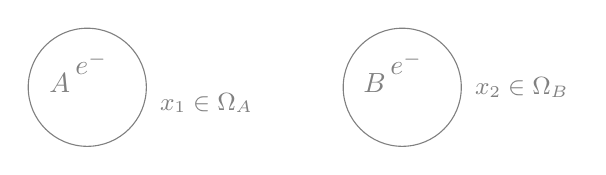
\begin{tikzpicture}[gray]
  \draw (0,0) circle (0.75);
  \node at (-0.35,0.05) {$A$}; \node at (0.05,0.3) {$e^-$};
  \node[right] at (0.8,-0.2) {\small $x_1\in\Omega_A$};
  \draw (4,0) circle (0.75);
  \node at (3.65,0.05) {$B$}; \node at (4.05,0.3) {$e^-$};
  \node[right] at (4.8,0) {\small $x_2\in\Omega_B$};
\end{tikzpicture}
\end{minipage}

vln.\ fce atomu $A$: \ $\phi_A(\vec x_1)$ \hfill vl.\ fce atomu $B$: \ $\phi_B(\vec x_2)$

vln.\ fce složeného systému: \quad
$\phi(x_1,x_2) = \frac{1}{\sqrt2}\big[\phi_A(x_1)\phi_B(x_2) \pm \phi_A(x_2)\phi_B(x_1)\big]$ \\
\hspace*{9cm} pro singlet / triplet.

\dots\ \pozor{MRZUTÉ!} \dots\ atom v laboratoři je promíchaný s atomem na Měsíci!? \\
naštěstí nemá pozorovatelné důsl., pokud $\Omega_A\cap\Omega_B = \emptyset$

Např.: hustota pravd.\ nalezení $e^-$ v $A$ a druhého v $B$: \ $x_1\in\Omega_A$, $x_2\in\Omega_B$
\begin{align*}
  p(x_1,x_2) = \tfrac12\Big\{&|\phi_A(x_1)|^2\cdot|\phi_B(x_2)|^2 + |\phi_A(x_2)|^2\cdot|\phi_B(x_1)|^2 \\
  &\pm \underbrace{2\,\mathrm{Re}\,\phi_A(x_1)\phi_B(x_2)\phi_A^*(x_2)\phi_B^*(x_1)}_{\text{výměnný člen}}\Big\}
\end{align*}
\quad výměnný člen \dots\ udělá pro $x_1 = x_2$ \quad hustotu \quad
$\begin{cases} 0 & \text{pro Fermiony} \\ 2\times\text{větší} & \text{pro Bosony}\end{cases}$

ale pro $x_1\in\Omega_A$, $x_2\in\Omega_B$ zbude jen $p_A\cdot p_B$

%----------------------------------------------------------------------
\strana{I4}
\subsection*{Atom Helia}
\[
  H = \frac{p_1^2}{2m} + \frac{p_2^2}{2m} - \frac{Ze^2}{r_1} - \frac{Ze^2}{r_2} + \boxed{\frac{e^2}{r_{12}}}
\]
řešení jako atom vodíku, ale $Z = 1\to Z = 2$

0.\ přiblížení: zanedbáme $e^-$--$e^-$ interakci $\uparrow$:
\[
  \phi(\vec x_1,\vec x_2) = \frac{1}{\sqrt2}\Big[\psi_{nlm}(\vec x_1)\psi_{n'l'm'}(\vec x_2) \pm \psi_{nlm}(\vec x_2)\psi_{n'l'm'}(\vec x_1)\Big]
  \qquad \pozn{$+$ pro singlet, $-$ pro triplet}
\]
speciálně základní stav \quad $n = n' = 1$, $l = l' = 0$, $m = m' = 0$ \dots\ dovoleno jen $+$
\[
  \phi_0(\vec x_1,\vec x_2) = \frac{Z^3}{\pi a_0^3}e^{-Z(r_1+r_2)/a_0}\cdot\chi_{\text{singlet}}
  \qquad \pozn{$\chi_{\text{singlet}} = \frac{1}{\sqrt2}\big(\ket{\uparrow\downarrow} - \ket{\downarrow\uparrow}\big)$}
\]
\hfill $E_0 = 2\times\Big(-\dfrac{4e^2}{2a_0}\Big) = -8\cdot\dfrac{e^2}{2a_0}$ \quad \pozn{$\sim -108.84$\,eV}

\begin{itemize}
  \item poruchová teorie \dots\ 1.\ korekce:
  \[
    \Delta_{(1s)^2} = \Big\langle\frac{e^2}{r_{12}}\Big\rangle_{\phi_0} = \iint\frac{Z^6}{\pi^2a_0^6}e^{-2Z(r_1+r_2)/a_0}\frac{e^2}{r_{12}}\,\dd^3x_1\,\dd^3x_2
  \]
  + použití multipól.\ rozvoje: \quad
  $\dfrac{1}{r_{12}} = \displaystyle\sum_{lm}\frac{4\pi}{2l+1}\frac{r_<^l}{r_>^{l+1}}Y_{lm}^*\Big(\frac{x_1}{r_1}\Big)Y_{lm}\Big(\frac{x_2}{r_2}\Big)$ \\
  + $\displaystyle\int\dd\Omega_{x_1}Y_{lm}\Big(\frac{x_1}{r_1}\Big) \sim \delta_{l0}\delta_{m0}$ -- zruší sumu \\
  ve shodě je třeba rozdělit $\int_0^\infty\!\int_0^\infty\dd r_1\dd r_2$ na $\int_0^\infty\Big[\int_0^{r_1} + \int_{r_1}^\infty\Big]$

  \dots\ $\Delta E = \frac52\Big(\dfrac{e^2}{2a_0}\Big)$ \quad \dots \quad
  $E = \Big(-8 + \frac52\Big)\Big(\dfrac{e^2}{2a_0}\Big) \doteq -74.8$\,eV

  \item Variační metoda: \\
  nejjednodušší vzít stejnou funkci, ale proměnné $Z'$ (screening) \\
  tj.\ \quad $\phi_v(\vec x_1,\vec x_2) = \dfrac{Z'^3}{\pi a_0^3}e^{-Z_{\text{eff}}(r_1+r_2)/a_0}$

  výpočet $E(Z') = \langle H\rangle_{\phi_v}$ probíhá jako $\uparrow$
  \[
    E(Z') = \langle T_0\rangle + \langle V_0\rangle + \Big\langle\frac{e^2}{r_{12}}\Big\rangle
    = \Big(2\frac{Z'^2}{2} - 2ZZ' + \frac58Z'\Big)\Big(\frac{e^2}{a_0}\Big)
  \]
  $\to$ minimum \quad $Z' = 2 - \frac{5}{16}$ \quad $\to$ \quad $\vzorec{E = -77.5\,\text{eV}}$ \\
  \hspace*{6.3cm} $E_{\text{exp}} \doteq -78.8$\,eV
\end{itemize}

\underline{Excit.\ stavy:} \quad $n'l'm' \neq (1,0,0)$
\[ E = E_{100} + E_{nlm} + \Delta E \]
v 1.\ řádu: \quad $\Delta E = \Big\langle\dfrac{e^2}{r_{12}}\Big\rangle = I \pm J$
\begin{align*}
  \text{přímá interakce}\quad I &= \int\dd^3x_1\int\dd^3x_2\,|\psi_{100}(x_1)|^2|\psi_{nlm}(x_2)|^2\frac{e^2}{r_{12}} \\
  \text{\kw{výměnný integrál}}\quad J &= \int\dd^3x_1\,\dd^3x_2\,\psi_{100}^*(\vec x_1)\psi_{nlm}^*(\vec x_2)\frac{e^2}{r_{12}}\psi_{100}(\vec x_2)\psi_{nlm}(\vec x_1) \\
  &\qquad\text{(single center)}
\end{align*}

%======================================================================
\strana{I5}
\section{Systémy identických částic -- rozvinutí formalismu}
\hfill (literatura: Formánek, Ballentine)

\underline{opakování} (shrnutí):
\begin{itemize}[nosep]
  \item[--] permutační (výměnná) symetrie
  \item[--] rozpad $\forall$ vl.\ podprostorů podle IR permutační grupy
  \item[--] symetrizační postulát $\to$ jen totálně symetrická / antisymetrická 1-D reprezentace se realizuje v přír.
\end{itemize}

\underline{závěr:} $\mathcal{H} = \mathcal{H}_1\otimes\mathcal{H}_2\otimes\dots\otimes\mathcal{H}_N$ není správným stav.\ prostorem pro systém ident.\ částic, ale jen jeho podprostor $\mathcal{H}_S/\mathcal{H}_A$

dva způsoby popisu \dots\ \textcircled{A} uvnitř $\mathcal{H}$ jako podprostor \\
\hspace*{3.8cm} \textcircled{B} elegantní formalismus \kw{Fockova prostoru}

\textcircled{A} Pro popis stavů používáme jen totálně symetrické (bosony) / totálně antisymetrické (fermiony) funkce z $\mathcal{H}$ \\
Popis měření \dots\ operátory na $\mathcal{H}$, ale správná veličina $[A,P_{ij}] = 0\ \ \forall i,j$

\underline{popis vektorů z $\mathcal{H}_S/\mathcal{H}_A$}

\dots\ úplná množina pozorovatelných na $\mathcal{H}_1\equiv\mathcal{H}_2\equiv\dots\equiv\mathcal{H}_N$ \\
\quad $\to$ \quad $\hat C = \sum_n c_n\ket{n}\bra{n}$ \quad \dots\ $\hat C\ket{n} = c_n\ket{n}$ \\
stavy z $\mathcal{H}$ \dots\ $\ket{n_1n_2\dots n_N} \equiv \ket{n_1}\otimes\ket{n_2}\otimes\dots\otimes\ket{n_N}$

permutace $p = \begin{pmatrix} 1 & 2 & \dots & n \\ p_1 & p_2 & \dots & p_n\end{pmatrix}$ \quad \dots\ operátor \quad
$\hat P_p\ket{n_1\dots n_N} = \ket{n_{p_1}\dots n_{p_N}}$ \\
\pozn{dosud jsme měli jen $P_{ij}$ \dots\ $\begin{pmatrix}1&2&\dots&i&\dots&j&\dots&n\\1&2&\dots&j&\dots&i&\dots&n\end{pmatrix} \equiv p_{ij}$}

totálně sym./antisym.\ vektory \quad $\hat P_p\ket{\psi} = \pm\ket{\psi}$ \quad $\leftarrow$ pro liché permutace

\begin{veta}[Projektory na $\mathcal{H}_S/\mathcal{H}_A$]
\[
  \hat S = \frac{1}{N!}\sum_p\hat P_p, \qquad
  \hat A = \frac{1}{N!}\sum_p(-1)^p\hat P_p \qquad (-1)^p\ \dots\ \text{znaménko permutace}
\]
\end{veta}

DK, že projektory \dots\ $\forall$ permutace lze složit z transpozic $\to$ $\hat P_p = \hat P_{ij}\dots\hat P_{i'j'}$ \\
\quad pro $P_{ij}$ víme \dots\ $P_{ij}^2 = I$, \quad $P_{ij}^\dagger = P_{ij}$ \quad $\Rightarrow$ \quad $S^\dagger = S$; \ $A^\dagger = A$ \\
\hspace*{9.5cm} (suma probíhá přes $p^{-1}$)

+ platí \quad
$\begin{aligned}[t]
  \hat P_{jk}\hat S &= \hat S\hat P_{jk} = \hat S \\
  \hat P_{jk}\hat A &= \hat A\hat P_{jk} = -\hat A
\end{aligned}$
\quad (suma přes $p_{jk}p$ \dots\ probíhá $\forall$ permutace)

$\Rightarrow$ \quad 1) \ $P_{jk}\ket{\phi} = +\ket{\phi}$ \ pro $\ket{\phi} = S\ket{\psi}$ \\
\hspace*{1.95cm} $= -\ket{\phi}$ \ \dots\ $\ket{\phi} = A\ket{\psi}$ \\[3pt]
\quad\quad 2) \ $\hat S^2 = \frac{1}{N!}\sum_p\hat P\hat S = \frac{1}{N!}N!\,\hat S$, \qquad
$\hat A^2 = \frac{1}{N!}\sum_p(-1)^p\hat P\hat A = \frac{1}{N!}N!\,(-1)^{2p}\hat A$

%----------------------------------------------------------------------
\strana{I6}
působení v $x$-reprezentaci \dots\ $\ket{\psi} = \ket{\phi_1}\ket{\phi_2}\dots\ket{\phi_N}$ \\
\hspace*{3.5cm} $\to$ \quad $\psi(x_1\dots x_N) \equiv \braket{x_1\dots x_N}{\psi} = \phi_1(x_1)\dots\phi_N(x_N)$

\quad 1) \quad $\hat P\psi = \phi_1(x_{p_1})\dots\phi_N(x_{p_N})$

\kw{Slaterův determinant}: \\
\quad 2) \quad
\[
  \mathcal{N}\cdot\hat A\psi \equiv \mathcal{N}\cdot\hat A\,\phi_1(x_1)\dots\phi_N(x_N)
  = \vzorec{\frac{1}{\sqrt{N!}}
  \begin{vmatrix}
    \phi_1(x_1) & \phi_1(x_2) & \dots & \phi_1(x_N) \\
    \phi_2(x_1) & & & \vdots \\
    \vdots & \vdots & & \\
    \phi_N(x_1) & \phi_N(x_2) & \dots & \phi_N(x_N)
  \end{vmatrix}}
\]
\quad $\mathcal{N}$ \dots\ normalizační koef.\ $\sqrt{N!}$

\subsection*{Reprezentace obsazovacích čísel}
problém \dots\ konstrukce báze \ $S\ket{n_1n_2\dots n_N}$ \quad \dots\ $\mathcal{H}\to\mathcal{H}_S$ \\
\hspace*{4.4cm} $\downarrow\ \ \dots\ \ \downarrow$ \\
\quad při procházení $\forall$ hodnot \quad $c_{n_1}\ \dots\ c_{n_N}$ \ operátoru $\hat C$ \\
\quad dostanu vektory \sout{s $n_1 = n_2$} vícekrát

např.\ \quad $S\ket{n_1\dots n_i\dots n_j\dots n_N} = S\ket{n_1\dots n_j\dots n_i\dots n_N}$

$S\ket{n_1\dots n_N}$ lze jednoznačně charakterizovat tzv.\ \kw{obsaz.\ čísly} \\
\quad $N_1, N_2,\dots$ \quad $N_1 + N_2 + \dots = N$ \quad \dots\ $N_i$ udává, kolikrát se vyskytuje \\
\hspace*{3cm} v $\ket{n_1\dots n_N}$ číslo $n_i$, tj.\ hodnota $c_{n_i}$ \\
\hspace*{3cm} \dots\ kolik částic má je ve stavu $\ket{n_i}$ \dots

\begin{definice}[obsazovací čísla]
tj.\ def \quad $\ket{N_1N_2\dots} = \mathcal{N}\hat S\ket{n_1\dots n_N}$, \quad kde číslo $n_i$ se vyskytuje $N_{n_i}$ krát
\end{definice}

např.\ \quad $\ket{10201\dots} = \mathcal{N}\hat S\ket{1335}$ \quad \pozn{+ rozvést \dots\ několik 1.\ stavů v obou značeních}

normalizační koeficient $\mathcal{N}$? \quad \dots \quad $\vzorec{\mathcal{N} = \sqrt{\frac{N!}{N_1!N_2!\dots}}}$

\underline{DK:} \quad
$\hat S\ket{n_1\dots n_N} = \Big(\dfrac{N!}{N_1!N_2!\dots}\ \text{navz.\ OG členů}\Big)\times\big(\text{faktor } N_1!N_2!\dots\big)\cdot\underbrace{\dfrac{1}{N!}}_{\text{z def } \hat S}$
\[
  \Rightarrow\quad \mathcal{N} = \sqrt{\frac{N_1!N_2!\dots}{N!}\cdot\frac{N!}{N_1!N_2!\dots}} = \ \nearrow
\]

relace úplnosti na $\mathcal{H}_S$ \dots \quad
$I\,(=\hat S) = \displaystyle\sum_{\substack{N_1N_2\dots \\ \sum N_k = N}}\ket{N_1N_2\dots}\bra{N_1N_2\dots}$

Fermiony \dots\ jediný rozdíl, že $N_i\in\{0,1\}$, jinak $\hat A\ket{n_1\dots n_N} = 0$
\[
  \Rightarrow\quad \ket{N_1N_2\dots} = \sqrt{N!}\,A\ket{n_1\dots n_N}
\]
\hrule\smallskip

pozn: relace úplnosti na $\mathcal{H}$: \quad
$\displaystyle\sum_{n_1n_2\dots n_N}\ket{n_1n_2\dots n_N}\bra{n_1\dots n_N} = 1_{\mathcal{H}}$ \quad $\Big\downarrow A(\cdot)A$
\[
  \sum_{n_1\dots n_N}\underbrace{A\ket{n_1\dots n_N}}_{\frac{1}{\sqrt{N!}}\ket{N_1N_2\dots}}\bra{n_1\dots n_N}A = A = 1_{\mathcal{H}_A}
\]
$\sum_{N_1N_2\dots}$, ale $\forall$ člen je tam $N!\times$ \quad $\to$ \quad
$N!\displaystyle\sum_{N_1N_2\dots}\Big(\frac{1}{\sqrt{N!}}\Big)^2\ket{N_1N_2\dots}\bra{N_1N_2\dots} = 1_{\mathcal{H}_A}$

podob.\ $\mathcal{H}_S$

%----------------------------------------------------------------------
\strana{I7}
\subsection*{Operátory ve Fokově (Fockově) prostoru}
\begin{minipage}{0.55\textwidth}
\underline{pozn:} Vladimir Alexandrovič Fok \pozn{v originále azbukou} \\
přepis do češtiny? FOK / FOCK?
\end{minipage}
\begin{minipage}{0.43\textwidth}
\underline{Google} (2011): \\
Hartree--Fock \dots\ cca 500\,000 \\
Hartree--Fok \dots\ cca 500 \\
Hartree--Fork \dots\ cca 3000
\end{minipage}

\begin{definice}[Fockův prostor]
\[
  \mathcal{H}_F \equiv \bigoplus_{N=0}^{\infty}\mathcal{H}_S^{(N)}, \quad\text{kde } \mathcal{H}_S^{(N)} \text{ je tot.\ sym.\ prostor } N \text{ částic}
\]
podob.\ \quad $\bigoplus_{N=0}^{\infty}\mathcal{H}_A^{(N)}$ \quad pro Fermiony
\end{definice}

\textcircled{1} \underline{případ Bosonů}

definitoricky $\mathcal{H}_S^{(0)}$ je 1D prostor s bází $\ket{0}$ \dots\ \kw{vakuum} \dots\ žádná částice \\
\hspace*{2.3cm} $\mathcal{H}_S^{(N)}$ \dots\ tot.\ sym.\ prostor s bází $\ket{N_1N_2\dots}$, \quad $N_1 + N_2 + \dots = N$

hodí se pro popis otevřených systémů nebo kreaci/anihilaci částic, ale výhody i pro fixní $N$ \dots\ algebraická struktura \\
\hspace*{3cm} $N_n$ \dots\ shodné spektrum jako nezáv.\ harm.\ oscil.

\begin{definice}[kreační operátor]
\kw{kreační operátor} $\hat a_n^\dagger$ částice ve stavu $\ket{n}$ \\
\hspace*{3cm} (nezapomínat \dots\ záv.\ na bázi $\hat C\ket{n} = c_n\ket{n}$) \\
$\hookrightarrow$ operátor na $\mathcal{H}_F$ \quad $a_n^\dagger: \mathcal{H}_S^{(N)}\to\mathcal{H}_S^{(N+1)}$
\[
  \vzorec{a_n^\dagger\ket{N_1\dots N_n\dots} = \sqrt{N_n+1}\,\ket{N_1\dots N_n+1\dots}}
  \qquad\dots\ \text{přidá částici do stavu } \ket{n}
\]
\end{definice}

\underline{vlastnosti:}
\begin{itemize}
  \item $\vzorec{a_n\ket{N_1\dots N_n\dots} = \sqrt{N_n}\,\ket{N_1\dots N_n-1\dots}}$ \quad \dots\ \kw{anihilační operátor} \\
        speciálně \quad $a_n\ket{0} = 0$ \\
        \pozn{DK: $\mel{N_1'\dots N_n'}{a_n^\dagger}{N_1\dots N_n\dots} = \mel{N_1\dots N_n\dots}{a_n}{N_1'\dots N_n'\dots}^*$}
  \item $\ket{N_1,N_2\dots} = \dfrac{1}{\sqrt{N_1!}}(a_1^\dagger)^{N_1}\dfrac{1}{\sqrt{N_2!}}(a_2^\dagger)^{N_2}\dots\ket{0}$ \\
        neboli \quad $S\ket{n_1}\dots\ket{n_N} = \dfrac{1}{\sqrt{N!}}a_{n_1}^\dagger\dots a_{n_N}^\dagger\ket{0}$ \quad
        \pozn{$= \sqrt{\frac{N_1!N_2!\dots}{N!}}\ket{N_1N_2\dots}$}
  \item $[a_i^\dagger,a_j^\dagger] = [a_i,a_j] = 0$ \qquad $\vzorec{[a_i,a_j^\dagger] = \delta_{ij}}$ \\
        \pozn{DK: $\uparrow$ je vidět z def.} \qquad
        \pozn{rovnež z def.\ -- pro $i = j$: \ $a_ia_i^\dagger\ket{N_1\dots N_i\dots} = (N_i+1)\ket{N_1\dots N_i\dots}$, \ $a_i^\dagger a_i\ket{N_1\dots N_i\dots} = N_i\ket{N_1\dots N_i\dots}$ \ $\forall N_1,N_2$}
  \item operátor počtu částic ve stavu $i$: \quad $\hat N_i = a_i^\dagger a_i$
  \item operátor celk.\ počtu částic \dots\ $\hat N = \sum_i\hat N_i$
\end{itemize}

%----------------------------------------------------------------------
\strana{I8}
\underline{změna báze:} \quad $\hat C\ket{n} = c_n\ket{n}$ \quad $\to$ \quad $\hat B\ket{b{:}n} = b_n\ket{b{:}n}$ \\
kreační operátory \quad $\ket{c{:}n} = \hat a_n^\dagger(c)\ket{0}$ \qquad $\ket{b{:}n} = \hat a_n^\dagger(b)\ket{0}$ \\
transformace báze \quad $\ket{b{:}n} = \sum_m\ket{c{:}m}\underbrace{\braket{c{:}m}{b{:}n}}_{\text{koef.\ rozvoje}}$
\[
  \Rightarrow\quad
  \left.\begin{aligned}
    \hat a_n^\dagger(b) &= \sum_m\hat a_m^\dagger(c)\braket{c{:}m}{b{:}n} \\
    \hat a_n(b) &= \sum_m\hat a_m(c)\braket{b{:}n}{c{:}m}
  \end{aligned}\right\}
  \ \to\ [\hat a_n(b),\hat a_m^\dagger(b)] = \delta_{nm}\ \ \text{díky unitaritě } \braket{c{:}m}{b{:}n}
\]

\underline{spojitá báze:} \quad $\braket{x}{n} = \phi_n(x)$ \quad \dots\ def.\ kreač.\ oper.\ $\psi^\dagger(x)\ket{0} = \ket{x}$
\[
  \Rightarrow\quad
  \left.\begin{aligned}
    \hat\psi^\dagger(x) &= \sum_n\hat a_n^\dagger\braket{n}{x} = \sum_n\phi_n(x)^*\hat a_n^\dagger \\
    \hat\psi(x) &= \sum_n\phi_n(x)\hat a_n
  \end{aligned}\right\}
  \quad\text{\uv{\kw{field operators}}}
\]
Podobně lze zahrnout spin \quad $\hat\psi_m^\dagger(x)\ket{0} = \ket{x}\ket{s,m}$ \\
operátor hustoty počtu částic v místě $x$: \quad $\hat N(x) = \hat\psi^\dagger(x)\hat\psi(x)$

\subsection*{Vyjádření operátorů}
\uv{\kw{Jednočásticový operátor}} na $\mathcal{H} = \mathcal{H}_1\otimes\dots\otimes\mathcal{H}_N$

příklad \quad $\hat{\mathbb{C}} = \sum_{i=1}^{N}\hat c^{(i)}$, \quad kde $\hat c^{(i)} \equiv \underset{1}{\hat 1}\otimes\dots\otimes\underset{i}{\hat c}\otimes\dots\otimes\underset{N}{\hat 1}$ \\
\quad $\uparrow$ ale jen \dots\ nemá smysl se ptát, jaké $\hat c$ naměřím na částici 1, (nerozlišitelnost)
\[
  \hat{\mathbb{C}}\ket{n_1}\ket{n_2}\dots\ket{n_N} = \underbrace{(c_{n_1} + c_{n_2} + \dots + c_{n_N})}_{\text{hodnota } c_{n_i} \text{ je zde } N_{n_i} \text{ krát}}\ket{n_1}\dots\ket{n_N}
  = \underbrace{(c_1N_1 + c_2N_2 + \dots)}_{\sum_ic_i\underbrace{\scriptstyle\hat a_i^\dagger\hat a_i}_{N_i}}\ket{n_1}\dots\ket{n_N}
\]
Symetrizace $\mathcal{N}\hat S\cdot$ \quad $[\hat{\mathbb{C}},\hat S] = 0$ \quad $\to$ \quad
$\hat{\mathbb{C}}\ket{N_1N_2\dots} = \sum_ic_i\hat a_i^\dagger\hat a_i\ket{N_1N_2\dots}$

tj.\ \quad $\hat{\mathbb{C}} = \sum_ic_i\hat a_i^\dagger\hat a_i$ \quad + přechod k jiné bázi \quad
$\hat a_i^\dagger(c) = \sum_j\hat a_j^\dagger(b)\braket{b{:}j}{c{:}i}$
\[
  \hat{\mathbb{C}} = \sum_{jj'}\underbrace{\sum_i\braket{b{:}j}{c{:}i}c_i\braket{c{:}i}{b{:}j'}}_{\mel{b{:}j}{\hat c}{b{:}j'}\equiv c_{jj'}}\hat a_j^\dagger\hat a_{j'}(b)
  \qquad\leftarrow\ \text{vyjádření nezáv.\ na bázi}
\]

\begin{veta}[Jednočásticový operátor ve Fockově prostoru]
tj.\ $\forall$ operátor $\hat{\mathbb{R}} \equiv \sum_i\hat r^{(i)}$: \quad
\[
  \vzorec{\hat{\mathbb{R}} = \sum_{nn'}\underbrace{\mel{n}{\hat r}{n'}}_{R_{nn'}}\hat a_n^\dagger\hat a_{n'}}
\]
$\uparrow$ vyjádření, které platí pro 1-čás.\ operátor bez ohledu na počet částic, tj.\ $\hat{\mathbb{R}} = \sum_{i=1}^{N}\hat r^{(i)}$ na $\forall\mathcal{H}_S^{(N)}\subset\mathcal{H}_F$
\end{veta}

%----------------------------------------------------------------------
\strana{I9}
Podobně \kw{dvoučásticový operátor}
\[
  \hat{\mathbb{R}} \equiv \sum_{i<j}\hat r^{(ij)}
  \quad\dots\ \text{ukážeme za chvíli pro fermiony}\quad
  \longrightarrow\ \frac12\sum_{klmn}\mel{kl}{\hat r^{(ij)}}{mn}\,a_k^\dagger a_l^\dagger a_n a_m
\]
\pozn{šipky: pořadí $m,n$ u anihilačních operátorů je obrácené}

\textcircled{2} \underline{případ Fermionů}
\[
  \mathcal{H}_F \equiv \bigoplus_{N=0}^{\infty}\mathcal{H}_A^{(N)}
\]
na $\forall\mathcal{H}_A^{(N)}$ báze (ortonormální) \quad $\ket{N_1,N_2\dots} \equiv \sqrt{N!}\,\hat A\ket{n_1n_2\dots n_N}$, \\
\hspace*{7.5cm} kde $N_1 + N_2 + \dots = N$ \\
pokud nepořadujeme $\nearrow$ máme bázi na celém $\mathcal{H}_F$

Pauliho princip \dots\ $N_i\in\{0,1\}$ \quad (jinak $\hat A\ket{n_1\dots n_N} = 0$ \dots\ pro $n_i = n_j$)

\begin{definice}[kreační operátor (fermiony)]
\[
  \left(\begin{aligned}
    b_n^\dagger\ket{N_1\dots N_n\dots} &= \sqrt{N_n}\,\ket{N_1\dots N_n+1\dots}\ ? \\
    b_n^\dagger\ket{N_1\dots N_n{=}0\dots} &= \ket{N_1\dots N_n{=}1\dots}\ ?
  \end{aligned}\right)\ \pozn{?}
\]
$\to$ ano, ale jen $N_n = 0$, tj.
\[
  \hat A\ket{n_1\dots n_N} = \frac{1}{\sqrt{N!}}b_{n_1}^\dagger\dots b_{n_N}^\dagger\ket{0} \qquad (*)
\]
\end{definice}
\[
  \hat A\ket{n_1\dots n_i\dots n_j\dots n_N} = -\hat A\ket{n_1\dots n_j\dots n_i\dots n_N}
  \qquad \boxed{\text{vzpomeň: } \hat P_{ij}\hat A = -\hat A}
\]
spec.\ pro dvoučástic.\ stavy: \quad
$\frac{1}{\sqrt2}b_n^\dagger b_m^\dagger\ket{0} = -\frac{1}{\sqrt2}b_m^\dagger b_n^\dagger\ket{0}$ \\
\hspace*{6cm} $\uparrow$ nemůžou komutovat
\begin{itemize}
  \item \dots\ relace \quad $\vzorec{\{b_i^\dagger,b_j^\dagger\} = 0}$ \quad $\leftarrow$ automaticky dá i splnění $\uparrow$ \\
        \hspace*{2.2cm} $\downarrow$
  \item \dots\ hermit.\ sdruž.\ \quad $\{b_i,b_j\} = 0$
\end{itemize}

\underline{pozn:}
\begin{itemize}[nosep]
  \item[--] relace $\{b_i^\dagger,b_j^\dagger\} = 0$ v sobě obsahuje $b_j^{\dagger 2} = 0$ \dots\ tj.\ $N_j < 2$
  \item[--] díky antikom.\ relaci je \quad
        $b_n^\dagger\ket{N_1\dots N_n{=}0\dots} = (-1)^{N_1+\dots+N_{n-1}}\ket{N_1\dots N_n{=}1\dots}$ \quad \pozn{$(*)$}
  \item[--] z $(*)$ plyne, že správně norm.\ vektor je prostě $b_{n_1}^\dagger\dots b_{n_N}^\dagger\ket{0}$, \\
        tj.\ vektory $\forall$ možné obsazení $n_1\dots n_N$ tvoří bázi v $\mathcal{H}_F$
\end{itemize}

\begin{itemize}
  \item \dots\ platí antikom.\ relace \quad $\vzorec{\{b_i,b_j^\dagger\} = \delta_{ij}}$
\end{itemize}
DK: hermit.\ sdruž.\ operátoru splní $(*)$:
\[
  b_n\ket{N_1\dots N_n\dots} = \begin{cases}
    0 & \dots\ \text{pro } N_n = 0 \\
    (-1)^{N_1+\dots+N_{n-1}}\ket{N_1\dots\underbrace{N_n-1}_{0}\dots}
  \end{cases}
\]
\[
  \Rightarrow\quad
  \left.\begin{aligned}
    b_nb_m^\dagger &= \pm\ket{\dots N_m{=}1\dots N_n{=}0\dots}\ \text{nebo } 0 \\
    b_m^\dagger b_n &= \mp\ket{\dots N_m{=}1\dots N_n{=}0\dots}\ \text{nebo } 0
  \end{aligned}\right\}
  \ \{b_n,b_m^\dagger\} = 0 \text{ pro } n\neq m
\]

%----------------------------------------------------------------------
\strana{I10}
zvlášť $n = m$:
\begin{align*}
  b_nb_n^\dagger\ket{N_1\dots N_n\dots} &= \begin{cases}
    0 & \text{pro } N_n = 1 \\
    \underbrace{(-1)^{2(N_1+\dots+N_{n-1})}}_{1}\ket{N_1\dots N_n\dots} & \text{pro } N_n = 0
  \end{cases} \\
  b_n^\dagger b_n\ket{N_1\dots N_n\dots} &= +1\ket{N_1\dots\overset{1}{N_n}\dots}\ \ \text{pro } N_n = 1 \\
  &= 0 \hspace{3.3cm} \text{pro } N_n = 0
\end{align*}
\[ \Rightarrow\quad \{b_n,b_m^\dagger\} = \delta_{nm} \]

\underline{pozn:} $\ket{N_1\dots N_n\dots}$ je vl.\ vektor $b_nb_n^\dagger$ s vl.\ hodn.\ $1 - N_n$ \\
\hspace*{3.6cm} a vl.\ vektor $b_n^\dagger b_n$ s vl.\ hodn.\ $N_n$ \\
\quad tj.\ operátor počtu částic opět \quad $\hat N = \sum_nb_n^\dagger b_n$

\underline{záměna báze} \dots\ projde stejně jako u bosonů: \quad $\tilde b_m^\dagger = \sum_nb_n^\dagger\braket{n}{\tilde m}$ \\
\quad kde 1-částic.\ báze $\hat C\ket{n} = c_n\ket{n}$ se nahradí $\hat{\tilde C}\ket{\tilde m} = \tilde c_m\ket{\tilde m}$

speciálně \uv{polní operátory} \quad $\hat\psi^\dagger(x) = \sum_nb_n^\dagger\braket{n}{x} = \sum_nb_n^\dagger\phi_n(x)^*$

komut.\ relace $\Rightarrow$ \quad
$\{\hat\psi^\dagger(x),\hat\psi^\dagger(x')\} = \{\hat\psi(x),\hat\psi(x')\} = 0$ \\
\hspace*{3.85cm} $\vzorec{\{\hat\psi(x),\hat\psi^\dagger(x')\} = \delta(x - x')}$

\underline{operátory:} \quad 1-částicový \quad
$\hat{\mathbb{R}} = \sum_i\hat r^{(i)} = \sum_{nn'}\underbrace{\mel{n}{\hat r}{n'}}_{R_{nn'}}\hat b_n^\dagger\hat b_{n'}$ \\
\hspace*{2.4cm} spočítáno v $\mathcal{H}^{(1)}$ \dots\ stejné $\forall\hat r^{(i)}$ $\nearrow$

2-částicová interakce: \quad např.\ coulomb.\ repulze \ $\sum_{i<j}\dfrac{e^2}{|r_i - r_j|}$ \\
obecně \quad $\hat{\mathbb{R}} = \sum_{i<j}\hat r^{(ij)}$; \quad kde $r^{(ij)}$ působí jen na částici $i$ a $j$

\begin{align*}
  \hat{\mathbb{R}}\ket{n\dots n_i\dots n_j\dots} &= \sum_{i<j}\mel{n_in_j}{\hat r^{(ij)}}{n_in_j}N_iN_j\ket{n\dots n_i\dots n_j\dots} \\
  \text{\pozn{přepis do báz.\ obsaz.\ čísel, vysvětlit detailně}}\quad
  &= \sum_{k<l}\mel{kl}{\hat r}{kl}\hat N_k\hat N_l\ket{\dots N_k\dots N_l\dots} \\
  &= \frac12\sum_{kl}\mel{kl}{\hat r}{kl}\,b_k^\dagger b_l^\dagger b_lb_k\ket{\dots}
\end{align*}
+ záměna báze \quad $b_k^\dagger = \sum_m\tilde b_m^\dagger\braket{m}{k}$ \\
\hspace*{3cm} $\ket{kl} = \sum_{m_1m_2}\braket{m_1}{k}\braket{m_2}{l}\ket{m_1m_2}$
\[
  \to\quad \hat{\mathbb{R}} = \frac12\sum_{\substack{m_1m_2\\ m_1'm_2'}}
  \underbrace{\Big(\sum_{kl}\braket{m_1}{k}\braket{m_2}{l}\mel{kl}{\hat r}{kl}\braket{k}{m_1'}\braket{l}{m_2'}\Big)}_{\mel{m_1m_2}{\hat r}{m_1'm_2'}}
  \tilde b_{m_1}^\dagger\tilde b_{m_2}^\dagger\tilde b_{m_2'}\tilde b_{m_1'}
\]

%----------------------------------------------------------------------
\strana{I11}
\begin{veta}[Dvoučásticový operátor ve Fockově prostoru]
tj.\ obecně \quad $\hat{\mathbb{R}} = \sum_{i<j}\hat r^{(ij)}$, \quad pak
\[
  \vzorec{\hat{\mathbb{R}} = \frac12\sum_{klmn}\mel{kl}{\hat r}{mn}\,\hat b_k^\dagger\hat b_l^\dagger\hat b_n\hat b_m}
\]
\pozn{pozn:} \quad $\longrightarrow\ ;\ \longrightarrow\ \longleftarrow$ \quad \pozor{pořadí operátorů!}
\end{veta}

\subsection*{Rovnice Hartree--Fock-ovy}
systém $N$ identických fermionů s Hamiltonianem
\[
  \hat H = \hat H_1 + \hat H_2 = \sum_{mn}h_{mn}b_m^\dagger b_n + \frac12\sum_{klmn}v_{kl,mn}b_k^\dagger b_l^\dagger b_nb_m
\]
\underline{Idea:} hledání nejlepší vln.\ funkce ve tvaru
$\underbrace{\overset{1}{\ket{\phi_1}}\overset{2}{\ket{\phi_2}}\dots\overset{N}{\ket{\phi_N}}}_{\ket{\psi}}$ \\
\quad + variační metoda \quad $\longrightarrow$ \ \kw{Hartree} \\
\quad \dots\ nezávislé částice i pro interagující systém, ale vidí \uv{\kw{střední pole}} \\
\quad \dots\ neobsahuje \uv{korelace}, aby $j$-tý elektron \uv{věděl}, kde je $i$-tý \dots\ $\phi_i(x_i)$ \\
\hspace*{9cm} muselo by $\phi_j(x_j,x_i)$

problém \dots\ $\ket{\psi}$ není správná fce pro fermiony, ale:
\[
  \ket{\psi} = \sqrt{N!}\,A\overset{1}{\ket{\phi_1}}\dots\overset{N}{\ket{\phi_N}} = b_{\phi_1}^\dagger\dots b_{\phi_N}^\dagger\ket{0}
  = \frac{1}{\sqrt{N!}}\begin{vmatrix}\phi_1(x_1) & \dots & \phi_1(x_N) \\ \vdots & & \vdots \\ \phi_N(x_1) & \dots & \phi_N(x_N)\end{vmatrix}
\]
tj.\ hledáme nejlepší $\ket{\psi}$ ve tvaru $\uparrow$ ve smyslu Ritz.\ var.\ principu.

abychom mohli užívat formalismus vybudovaný výše, musí navíc
\begin{align*}
  \int\phi_n^*\phi_m \equiv \braket{n}{m} = \delta_{nm} &\quad\dots\ \text{vedlejší podmínka} \\
  \equiv \braket{\phi_n}{\phi_m} &\quad\dots\ \text{minimalizace funkcionálu s vazbou}
\end{align*}

\textcircled{1} \underline{Funkcionál energie}
\[
  E[\phi_1,\phi_2,\dots] = \mel{\psi}{H}{\psi} = \sum_n\big[\mel{\psi}{H_1}{\psi} + \mel{\psi}{H_2}{\psi}\big]
\]
\begin{align*}
  \mel{\psi}{H_1}{\psi} &= \bra{0}b_N\dots b_1\Big(\sum_{mn}^{\infty}h_{mn}b_m^\dagger b_n\Big)b_1^\dagger\dots b_N^\dagger\ket{0} \\
  &= \bra{0}\sum_{m,n=0}^{N}b_m\,h_{mn}b_m^\dagger b_n\,b_n^\dagger\ket{0} \\
  &= \sum_{n=0}^{N}h_{nn}\bra{0}b_n\underbrace{b_n^\dagger b_n}_{N_n}b_n^\dagger\ket{0} = \sum_{n=0}^{N}h_{nn} \equiv \sum_n\mel{\phi_n}{\hat h}{\phi_n}
\end{align*}
podob.
\begin{align*}
  \mel{\psi}{H_2}{\psi} &= \frac12\sum_{klmn}v_{kl,mn}\bra{0}b_N\dots b_1\big(b_k^\dagger b_l^\dagger b_nb_m\big)b_1^\dagger\dots b_N^\dagger\ket{0}
  \quad\text{musí } n,m\in\{1\dots N\} \\
  \text{+ musí být vypárované:}\quad
  &\frac12\sum_{klmn}v_{kl,mn}\big\{\delta_{ln}\delta_{km} + \delta_{lm}\delta_{kn}\big\}\bra{0}b_kb_lb_k^\dagger b_l^\dagger b_nb_mb_l^\dagger b_k^\dagger\ket{0}
\end{align*}

%----------------------------------------------------------------------
\strana{I12}
\begin{align*}
  \text{a)}\quad &\bra{0}b_kb_lb_k^\dagger b_l^\dagger\,\textcolor{red}{\underline{b_lb_k}}\,b_l^\dagger b_k^\dagger\ket{0} = \\
  &\qquad \underbrace{(\delta_{kl} - b_l^\dagger b_k)b_k^\dagger\ket{0} = \delta_{kl}b_k^\dagger\ket{0} - b_l^\dagger\ket{0}}_{\delta_{kl}\ket{0} - \ket{0}\ =\ \ket{0}(\delta_{kl} - 1)} \\
  &= (\delta_{kl} - 1)\bra{0}b_kb_lb_k^\dagger b_l^\dagger\ket{0} = (1 - \delta_{kl}) \\[4pt]
  \text{b)}\quad &\bra{0}b_kb_lb_k^\dagger b_l^\dagger\,\textcolor{red}{\underline{b_kb_l}}\,b_l^\dagger b_k^\dagger\ket{0} = (\delta_{kl} - 1)
  \qquad \textcolor{red}{\nwarrow\ \text{liší se jen pořadí}}
\end{align*}
\[
  \text{tj.:}\quad \mel{\psi}{H_2}{\psi} = \frac12\sum_{kl}\big(v_{kl,kl} - v_{kl,lk}\big)
  = \frac12\sum_{kl}\bra{\phi_k\phi_l}\hat v\big(\ket{\phi_k}\ket{\phi_l} - \ket{\phi_l}\ket{\phi_k}\big)
\]

vedlejší podmínka $\braket{\phi_k}{\phi_l} = \delta_{kl}$ \quad $\to$ Lagrangeovy multiplik.\ $\varepsilon_{kl}$ \\
$\to$ minimalizace funkcionálu $E[\phi_1\dots\phi_N] = \mel{\psi}{H}{\psi}$ za podmínky $\uparrow$

\pozn{mezivýsl.\ -- funkcionál}
\[
  \to\quad \delta\Big[\underbrace{\sum_n^N\mel{\phi_n}{\hat h}{\phi_n}}_{\textcolor{OliveGreen}{\textcircled{\scriptsize 1}}}
  + \underbrace{\frac12\sum_{kl}^N\bra{\phi_k}\bra{\phi_l}\hat v\big(\ket{\phi_k}\ket{\phi_l} - \ket{\phi_l}\ket{\phi_k}\big)}_{\textcolor{OliveGreen}{\textcircled{\scriptsize 2}}}
  - \underbrace{\sum_{kl}^N\varepsilon_{kl}\braket{\phi_k}{\phi_l}}_{\textcolor{OliveGreen}{\textcircled{\scriptsize 3}}}\Big] = 0
\]
změna do prvního řádu při záměně $\ket{\phi_n}\to\ket{\phi_n} + \ket{\delta\phi_n}$:

\textcolor{OliveGreen}{\textcircled{1}} \quad $\delta\sum_n\mel{\phi_n}{\hat h}{\phi_n} = \sum_n\mel{\delta\phi_n}{\hat h}{\phi_n} + \text{c.c.}$

\textcolor{OliveGreen}{\textcircled{2}}
\begin{align*}
  \delta\,\frac12\sum_{kl}\bra{\phi_k}\bra{\phi_l}\hat v\big(\ket{\phi_k}\ket{\phi_l} - \ket{\phi_l}\ket{\phi_k}\big)
  &= \frac12\sum_{kl}\bra{\delta\phi_k}\bra{\phi_l}\hat v\big(\ket{\phi_k\phi_l} - \ket{\phi_l\phi_k}\big) + \text{c.c.} \\
  &\quad + \frac12\sum_{kl}\bra{\phi_k}\bra{\delta\phi_l}\hat v\big(\ket{\phi_k\phi_l} - \ket{\phi_l\phi_k}\big)
\end{align*}
+ symetrie výměnná: \quad
$\bra{\phi}\bra{\psi}\hat v\hat P_{12}\ket{\phi'}\ket{\psi'} = \bra{\phi}\bra{\psi}\hat v\ket{\psi'}\ket{\phi'}$ \\
\hspace*{4.25cm} $= \bra{\phi}\bra{\psi}\hat P_{12}\hat v\ket{\phi'}\ket{\psi'} = \bra{\psi}\bra{\phi}\hat v\ket{\phi'}\ket{\psi'}$ \\
\hspace*{9cm} tj.\ možno současně vyměnit bra i kety \\
+ přeznačení sčít.\ proměnné
\[
  = \sum_{kl}\bra{\delta\phi_k}\bra{\phi_l}\hat v\big(\ket{\phi_k}\ket{\phi_l} - \ket{\phi_l}\ket{\phi_k}\big) + \text{c.c.}
\]

\textcolor{OliveGreen}{\textcircled{3}} \quad člen $\sum_{kl}^N\varepsilon_{kl}\braket{\phi_k}{\phi_l}$ \dots\ jistě máme volbu, $\sum_lU_{kl}\ket{\phi_l}$ změní \\
\quad bázi, ale ta nezmění determinant $A\ket{\phi_1}\dots\ket{\phi_N}$ \\
\quad tj.\ $\exists$ báze, kde \quad $\longrightarrow$ \quad $\sum_k\varepsilon_k\braket{\phi_k}{\phi_k}$

%----------------------------------------------------------------------
\strana{I13}
tj.\ \quad $\delta\sum_k\varepsilon_k\braket{\phi_k}{\phi_k} = \sum_k\varepsilon_k\braket{\delta\phi_k}{\phi_k} + \text{c.c.}$

tj.\ DOHROMADY \quad $\delta(\dots) = 0$ \quad \dots\ \textcolor{OliveGreen}{\textcircled{1}+\textcircled{2}+\textcircled{3}} $\to$

\begin{veta}[Rovnice Hartree--Foka (Hartree--Fock equation)]
\[
  \vzorec{\hat h\ket{\phi_k} + \sum_{\substack{l=1\\ l\neq k}}^{N}\bra{\phi_l^{(2)}}\hat v^{(12)}\Big(\ket{\phi_k^{(1)}}\ket{\phi_l^{(2)}} - \ket{\phi_l^{(1)}}\ket{\phi_k^{(2)}}\Big) = \epsilon_k\ket{\phi_k}}
\]
\textcolor{OliveGreen}{\small $\uparrow$ čísla označují přiřazení 2-částic.\ operátoru $v^{(12)}$}

lze interpretovat jako \fbox{$\hat H_{HF}\ket{\phi_k} = \epsilon_k\ket{\phi_k}$}, ale lépe uvidíme ze zápisu v konkrétní bázi:
\end{veta}

původní 1-částicová báze \dots\ $\hat c\ket{n} = c_n\ket{n}$ \dots\ kreač.\ oper.\ $\bar b_n^\dagger$ \\
nová báze v 1-částic.\ prostoru \ $\hat H_{HF}\ket{\phi_k} = \epsilon_k\ket{\phi_k}$ \dots\ \hspace{1.2cm} $b_k^\dagger$

\underline{připomenout:} H--F rovnice \dots\ podmínka, aby $b_1^\dagger\dots b_N^\dagger\ket{0}$ bylo nejlepší \\
\hspace*{2.7cm} řešení mnohočást.\ S.R.\ ve smyslu var.\ principu

zápis HF rovnic v pův.\ bázi: \quad
$\hat H_1 = \displaystyle\sum_{mn}^{\infty}\bar h_{mn}\bar b_m^\dagger\bar b_n$ \\
\hspace*{5cm} $\hat H_2 = \displaystyle\sum_{mnm'n'}^{\infty}\bar v_{mn,m'n'}\bar b_m^\dagger\bar b_n^\dagger\bar b_{n'}\bar b_{m'}$
\[
  \ket{\phi_k} = \sum_m^{\infty}\ket{m}\braket{m}{\phi_k}
\]
\begin{align*}
  \Rightarrow\quad H_{mn}^{(HF)} \equiv \mel{m}{\hat H_{HF}}{n} = \bar h_{mn}
  &+ \underbrace{\sum_{l=1}^{N}\sum_{m_1m_2}^{\infty}\bar v_{mm_1,nm_2}\braket{m_2}{\phi_l}\braket{\phi_l}{m_1}}_{\textcolor{OliveGreen}{\text{přímá interakce}}} \\
  &- \underbrace{\sum_{l=1}^{N}\sum_{m_1m_2}^{\infty}\bar v_{mm_1,m_2n}\braket{m_2}{\phi_l}\braket{\phi_l}{m_1}}_{\textcolor{OliveGreen}{\text{výměnná interakce}}}
\end{align*}
\hspace*{3.5cm} $\uparrow$ mohu psát $l$ jen $l\neq k$

\textcolor{OliveGreen}{operátor 1-částicové hustoty:} \quad $\hat\rho = \sum_l\ket{\phi_l}\bra{\phi_l}$ \quad \textcolor{OliveGreen}{$\to$ (výskyt výše)}

\underline{interpretace H-F rovnic:} \quad
$\hat H_{HF}\underbrace{\ket{\phi_k}}_{\textcolor{OliveGreen}{\text{orbitaly}}} = \underbrace{\epsilon_k}_{\textcolor{OliveGreen}{\text{1-čás.\ energie}}}\ket{\phi_k}$ \\
\hspace*{3.9cm} \textcolor{OliveGreen}{1-částicové vln.\ fce $\equiv$ orbitaly}

\pozor{pozor:} variační ($\equiv$ celková) energie: \\
\dots\ hezčí v bázi $\ket{\phi_k}$ \dots\ \quad
$v_{kl,k'l'} \equiv \sum\braket{\phi_k}{m}\braket{\phi_l}{n}\bar v_{mn,m'n'}\braket{m'}{\phi_{k'}}\braket{n'}{\phi_{l'}}$ \\
viz předch.\ str.\ \dots \quad
$\vzorec{E = \sum_{n=1}^{N}\epsilon_n - \frac12\sum_{nl=1}^{N}\big(v_{nl,nl} - v_{nl,ln}\big)}$ \\
\hspace*{6.5cm} \textcolor{OliveGreen}{$\uparrow$ korekce na část započtenou $2\times$}

$\hat H_{HF}[\hat\rho]$ \dots\ obsahuje 1-část.\ hamiltonián $\hat h$ \\
\quad \dots\ a \kw{střední pole} skládající se z přímé a výměn.\ části

problém: $\hat H_{HF}$ závisí na $\hat\rho \equiv \sum_l\ket{\phi_l}\bra{\phi_l}$, ale $\ket{\phi_l}$ řešením pro $H_{HF}$ \\
\quad \dots\ \kw{selfkonsistentní úloha} \quad \dots\ iterace

startovací hodnota \dots\ např.\ řešení jen pro $\hat H_1$ \\
\textcircled{1} najít $\forall\ket{\phi_k}$, $\epsilon_k$ pro dané $H_{HF}[\rho]$ \quad
\textcircled{2} považovat nejnižší $\epsilon_k$ za obsazené a spočíst nové $H_{HF}[\rho]$ a pokračovat na \textcircled{1}, dokud nezkonverguje

%----------------------------------------------------------------------
\strana{I14}
\subsection*{HF-rovnice v $x$-reprezentaci}
částice se spinem $\frac12$ \dots\ báze $\ket{x\sigma}$; \ $\sigma = \pm\frac12$ \\
výsledné jednočásticové stavy \dots\ $\phi_{k\sigma}(x) \equiv \braket{x\sigma}{\phi_{k\sigma}}$ \\
pro jednoduchost uvažujme spin.\ nezáv.\ interakci
\[
  \left.\begin{aligned}
    \hat h &= \frac{\hat p^2}{2m} + V(\hat x) \\
    \hat v^{(12)} &= v\big(\hat x_1^{(1)} - \hat x_2^{(2)}\big)
  \end{aligned}\right\}
  \ \Rightarrow\ \mel{x}{H^{(HF)}}{\phi_{k\sigma}}:
\]
\begin{align*}
  \Big[-\frac{\hbar^2}{2m}\Delta_x + V(x) + \int v(x - x')\rho(x')\,\dd x'\Big]\phi_{k\sigma}(x)& \\
  - \sum_l\phi_{l\sigma}(x)\int\phi_{l\sigma}^*(x')v(x - x')\phi_{k\sigma}(x')\,\dd x' &= \epsilon_k\phi_{k\sigma}(x)
\end{align*}
kde \quad $\rho(x) \equiv \sum_{l\sigma}^{N}|\phi_{l\sigma}(x)|^2$ \quad \dots\ jednočásticová hustota

\pozn{pozn: \ $v_{mm_1,nm_2} \equiv \bra{x\sigma}\bra{x_1\sigma_1}v\big(\hat x^{(1)} - \hat x^{(2)}\big)\ket{x'\sigma'}\ket{x_2\sigma_2} = \delta(x - x')\delta_{\sigma\sigma'}\delta(x_1 - x_2)\delta_{\sigma_1\sigma_2}$}

\underline{interpretace:}
\begin{itemize}[nosep]
  \item přímý člen má význam interakce s oblakem okolních nábojů s hustotou $\rho(x)$
  \item výměnný člen $\leftarrow$ přispívají jen $\phi_{l\sigma}$ se stejným spinem \\
        člen je \pozor{nelokální v $x$!}
\end{itemize}

\underline{Poznámky:} \quad metody typu \uv{\kw{meanfield}} \quad \dots\ teorie středního pole
\begin{itemize}
  \item stejný přístup se dá uplatnit pro
  \begin{enumerate}[label=(\alph*)]
    \item rozlišitelné částice \dots\ \kw{Hartree-ho rovnice} \\
          -- stejná rovnice, bez výměnného členu
    \item nerozlišitelné bosony \dots\ \underline{\kw{Gross--Pitaevskii} rovnice} \\
          speciálně pro základní stav obsazena jen nejnižší hladina \dots\ $\forall N$ elektrony v jediném $\psi_0(x)$, tj.\ výměnný člen nepřispívá (měl by znaménko $+$)
  \end{enumerate}
\end{itemize}
\[
  \vzorec{\Big[-\frac{\hbar^2}{2m}\Delta_x + V(x)\Big]\psi_0(x) + \Big[\int|\psi_0(x')|^2v(x - x')\,\dd x'\Big]\psi_0(x) = \epsilon_0\psi_0(x)}
\]
\hspace*{5cm} \textcolor{OliveGreen}{$\uparrow$ \uv{nelineární Schrödingerova rovnice}}

$\psi_0(x)$ \dots\ \uv{\kw{makroskopická vln.\ fce}} \quad \dots\ $\forall N$ částic ve stej.\ stavu \\
\hspace*{9.3cm} (v principu mnoho)

